%! TEX root = Geometria.tex

\documentclass{./Geometria.tex}

\begin{document}
\chapter{Espacio Afín Euclídeo}
Un espacio afín es euclídeo al incluir el \textbf{producto escalar}:
\begin{defin}
El producto escalar, que definimos como $<x,y> = x\cdot y$, nos permite medir distancias, entre otras cosas. Esto pasa a ser
\[
	\vb{x}\cdot \vb{y} = \sum x_{i}y_{i}
\]
Esta es una aplicación:
\[
	\cdot : \mathbb{R}^{n}\times \mathbb{R}^{n} \to \mathbb{R}
\]
Este cumple que:
\begin{itemize}
	\item Es simétrico.
	\item Es positivo siempre.
	\item Es una forma bilineal.
\end{itemize}
Figura \ref{fig:p-escalar}
\end{defin}
\begin{figure}[ht]
    \centering
    \incfig{p-escalar}
    \caption{Producto Escalar}
    \label{fig:p-escalar}
\end{figure}
Y ahora
\begin{defin}
Un espacio afín euclídeo es una cuaterna definida por $(A, \mathbb{V}, \phi, \cdot )$, formado por un espacio afín y el producto escalar.\\
La dimensión del EA euclídeo es la dimensión de su EA asociado.
\end{defin}
\section{Coordenadas covariantes y contravariantes}
\begin{defin}
	Dado un EA euclídeo sobre $\mathbb{R}$, con una base $\mathcal{B}= \{ \vb{v}_{i} \}$, llamamos \textbf{coordenadas contravariantes} del vector $\vb{u}\in E$, respecto a la base $\mathcal{B}$, a la $n$-upla $(a_1,\dots ,a_{n})$ de escalares tal que:
	\[
		\vb{u} = \sum^{n}_{i=1} a_{i} \vb{v}_{i}
	\]
\end{defin}
Por contraste, tenemos
\pagebreak
\begin{defin}
	Dado un EA euclídeo, las \textbf{coordenadas covariantes} de un vector $\vb{u}$, respecto a una base $\mathcal{B} = \{ \vb{v}_{i} \}$, son la $n$-upla definida por los escalares $(a^{*}_{1},\dots ,a^{*}_{n})$:
	\[
		a^{*}_{i} = \vb{v}_{i}\cdot \vb{u}
	\]
	Figura \ref{fig:coords-covariantes}\\
Lo importante de estas coordenadas, es que
\[
	<u_1,u_2><u_1^{*},u_2^{*}> = c
\]
Es decir, el producto de coordenadas covariantes entre coordenadas contravariantes es constante. Además, se cumplirá que si la base es ortonormal, ambas coincidirán.
\end{defin}
\begin{figure}[ht]
    \centering
    \incfig{coords-covariantes}
    \caption{Coordenadas Covariantes}
    \label{fig:coords-covariantes}
\end{figure}
Las coordenadas covariantes se pueden obtener multiplicando las coordenadas contravariantes por la \textbf{matriz de Gram}:
\[
	\begin{pmatrix} a_1^{*}\\\dots \\ a_{n}^{*} \end{pmatrix}=
	\begin{pmatrix} g_{11} & \dots & g_{1n}\\
		\dots & \dots &\dots \\
		g_{n 1} & \dots & g_{nn}
	\end{pmatrix} \begin{pmatrix} a_1\\ \dots \\ a_{n} \end{pmatrix} 
\]
\pagebreak
\section{Ángulos}
\begin{defin}
	Dado un EA euclídeo, y dos vectores $\vb{v}_{1}, \vb{v}_{2}$ no nulos, definimos el ángulo no orientado entre $\vb{v}_{1}$ y $\vb{v}_{2}$ como el $\arccos$ entre $0$ y $\pi$ de
	\[
		\cos \theta = \frac{\vb{v}_{1}\cdot \vb{v}_{2}}{|\vb{v}_{1}||\vb{v}_{2}|}
	\]
	Donde $|\vb{v}|$ es la norma del vector, definido como
	\[
		|\vb{v}| = \sqrt{\vb{v}\cdot \vb{v}}
	\]
\end{defin}
\begin{defin}[Perpendicularidad]
	Dado un EAE de dimensión $n$, y dos vectores $\vb{v}, \vb{u}$, estos dos son perpendiculares u ortogonales si y solo si
	\[
		\vb{v}\cdot \vb{u} = 0
	\]
	También, dos variedades afines $L_1=P_1+S_1$, $L_2=P_2+S_2$, estos serán perpendiculares si se cumple que:
	\begin{itemize}
		\item $L_1 \cap L_2 \neq \phi$
		\item $S_1 \perp S_2$ 
	\end{itemize}
\end{defin}
Ahora introducimos el siguiente teorema
\pagebreak
\begin{teorema}
	Dado un hiperplano $L$ cuya ecuación cartesiana respecto a un sistema rectangular (ortonormal), es
	\[
		\sum a_{i}x_{i} = c
	\]
	El vector de coordenadas $\vb{n} = (a_1,\dots ,a_{n})$ define rectas perpendiculares a $L$ y es el vector normal al hiperplano. Estas coordenadas son las \textbf{covariantes} del vector normal.  
\end{teorema}
\begin{defin}
	Dado un EAE de dimensión $n$, y un subespacio afín $L \subset A$ de dimensión $m$ y dirección $W$, entonces, para cada punto $P \in A$, existe un único subespacio afín $L'$ de $A$ por $P$, ortogonal a $L$ y con dimensión $n-m$. Este es
	\[
		L' = P + W^{\perp}
	\]
	La intersección entre ambas variadades, $L \cap L'$, es la proyección de $P$ sobre $L$.   
\end{defin}
\begin{figure}[ht]
    \centering
    \incfig{p-ortogonal}
    \caption{Proyección Ortogonal}
    \label{fig:p-ortogonal}
\end{figure}
\pagebreak
\section{Distancias}
\subsection{Distancia entre dos puntos}
\begin{defin}
Dado un EAE, y dos puntos $P,Q \in A$, la distancia entre los dos puntos es la norma del vector $\vb{PQ}$:
\[
	d(P,Q) = \norm{\vb{PQ}}
\]
Propiedades:
\begin{itemize}
	\item $d$ es definida positiva.
	\item $d$ es simétrica: $d(P,Q) = d(Q,P)$.
	\item $d$ cumple la desigualdad triangular: $d(P,Q) \leq d(P,R) + d(R,Q)$. 
\end{itemize}
\end{defin}
\subsection{Distancia entre variedades}
\begin{defin}
Dadas dos variedades $L_1=P_1+S_1$ y $L_2=P_2+S_2$, se define la distancia entre ellas como la menor distancia entre sus respectivos puntos:
\[
	d(L_1,L_2) = min(\{ d(X,Y) : X \in L_1, y \in L_2 \})
\]
Si se da que $L_1 \cap L_2 \neq \phi, d(L_1,L_2) = 0$.
\end{defin}
\subsection{Distancia entre punto y subespacio afín}
\begin{defin}
Dado un punto $P$ y un subespacio afín $L$, la distancia entre ambos es la distancia entre $P$ y la proyección ortogonal de $P$ y $L$:
\[
	d(P,L)= d(P,P_{L})
\]
\end{defin}
\section{Isometría}
\begin{defin}
Dados dos EAEs $(E, V, \phi)$ y $(E', V', \phi')$, diremos que una aplicación $f$ es una isometría si:
\begin{equation}
	\begin{split}
		f&: E \to E'\\
		(P,Q) &\to f(P,Q)
	\end{split}
\end{equation}
Y se debe cumplir que
\[
	\boxed{
		d'(f(P),f(Q)) = d(P,Q)
	}
\]
Donde $d$ es la distancia definida en $E$ y $d'$ es la distancia definida en $E'$.    
\end{defin}
\begin{center}
	

\end{center}
\begin{figure}[ht]
	\centering
	\caption{Isometrías}
	\label{fig:isometrias}


\tikzset{every picture/.style={line width=0.75pt}} %set default line width to 0.75pt

\begin{tikzpicture}[x=0.75pt,y=0.75pt,yscale=-1,xscale=1]
%uncomment if require: \path (0,300); %set diagram left start at 0, and has height of 300

%Shape: Ellipse [id:dp16206097342092396]
\draw   (90.2,157.19) .. controls (90.2,108.52) and (113.22,69.06) .. (141.61,69.06) .. controls (170,69.06) and (193.01,108.52) .. (193.01,157.19) .. controls (193.01,205.86) and (170,245.32) .. (141.61,245.32) .. controls (113.22,245.32) and (90.2,205.86) .. (90.2,157.19) -- cycle ;
%Shape: Ellipse [id:dp3924000237283274]
\draw   (405.99,152.78) .. controls (405.99,104.11) and (429,64.66) .. (457.39,64.66) .. controls (485.78,64.66) and (508.8,104.11) .. (508.8,152.78) .. controls (508.8,201.45) and (485.78,240.91) .. (457.39,240.91) .. controls (429,240.91) and (405.99,201.45) .. (405.99,152.78) -- cycle ;
%Straight Lines [id:da7556011380605056]
\draw    (163.34,117.53) -- (428.66,113.16) ;
\draw [shift={(430.66,113.13)}, rotate = 179.06] [color={rgb, 255:red, 0; green, 0; blue, 0 }  ][line width=0.75]    (10.93,-3.29) .. controls (6.95,-1.4) and (3.31,-0.3) .. (0,0) .. controls (3.31,0.3) and (6.95,1.4) .. (10.93,3.29)   ;
%Straight Lines [id:da5411924729180644]
\draw    (154.53,196.85) -- (419.85,196.85) ;
\draw [shift={(421.85,196.85)}, rotate = 180] [color={rgb, 255:red, 0; green, 0; blue, 0 }  ][line width=0.75]    (10.93,-3.29) .. controls (6.95,-1.4) and (3.31,-0.3) .. (0,0) .. controls (3.31,0.3) and (6.95,1.4) .. (10.93,3.29)   ;
%Straight Lines [id:da9279665366462678]
\draw    (142.8,121.85) -- (137.99,172.86) ;
\draw [shift={(137.8,174.85)}, rotate = 275.39] [color={rgb, 255:red, 0; green, 0; blue, 0 }  ][line width=0.75]    (10.93,-3.29) .. controls (6.95,-1.4) and (3.31,-0.3) .. (0,0) .. controls (3.31,0.3) and (6.95,1.4) .. (10.93,3.29)   ;
%Straight Lines [id:da36632798481514883]
\draw    (459.89,126.28) -- (457.88,177.85) ;
\draw [shift={(457.8,179.85)}, rotate = 272.24] [color={rgb, 255:red, 0; green, 0; blue, 0 }  ][line width=0.75]    (10.93,-3.29) .. controls (6.95,-1.4) and (3.31,-0.3) .. (0,0) .. controls (3.31,0.3) and (6.95,1.4) .. (10.93,3.29)   ;

% Text Node
\draw (133.86,44.09) node [anchor=north west][inner sep=0.75pt]    {$E$};
% Text Node
\draw (451.03,40.62) node [anchor=north west][inner sep=0.75pt]    {$E'$};
% Text Node
\draw (138.54,107.22) node [anchor=north west][inner sep=0.75pt]    {$P$};
% Text Node
\draw (130.44,180.65) node [anchor=north west][inner sep=0.75pt]    {$Q$};
% Text Node
\draw (441.39,104.28) node [anchor=north west][inner sep=0.75pt]    {$f( P)$};
% Text Node
\draw (437.69,182.12) node [anchor=north west][inner sep=0.75pt]    {$f( Q)$};


\end{tikzpicture}

\end{figure}
\textbf{Propiedades}:
\begin{itemize}
	\item La composición de isometrías una isometría.
	\item Las isometrías afines consevan los ángulos entre subespacios afines:
		\[
			\cos (\vb{u}, \vb{v}) = \cos (\bar{f}(\vb{u}), \bar{f}(\vb{v}))
		\]
\end{itemize}
\section{Ejemplos de transformaciones}
\begin{defin}
Una traslación por el vector $\vb{v}$ es una transformación afín que lleva un punto $P$ al punto $P + \vb{v}$.
\[
	P \mapsto t(P) = P+\vb{v}
\]
\end{defin}
\begin{defin}[Proyección ortogonal]
La aplicación
\[
	\delta:A \mapsto A
\]
\[
	P \mapsto \delta(P)
\]
donde $\delta(P)$ es el único punto del conjunto $L \cap L'$, y es una proyección. $\delta(P)$ es la proyección sobre $L$ con dirección $W^{\perp}$, y su aplicación lineal asociada es la proyección vectorial ortogonal sobre $W$.
\end{defin}
\pagebreak
\begin{defin}[Homotecia]
Sea $(E, V, \phi)$ un EAE, y sea $\lambda \in K - \{ 0,1 \}$, y sea un punto $O \in A$. Una homotecia es una aplicación $h: E \to E$ que deja $O$ fijo, y que tiene por aplicación lineal asociada una homotecia vertical de razón $\lambda$:
\begin{equation}
	\begin{split}
		h&: E \mapsto E\\
		P &\mapsto O + \lambda \vb{OP}
	\end{split}
\end{equation}
$h$ es una homotecia de razón $\lambda$ y centro $O$.\\
Si es una homotecia, la aplicación afín asociada de la homotecia es:
\[
	\bar{h} = \lambda Id
\]
Donde $\lambda$ es la razón de la homotecia.\\
Propiedades:
\begin{itemize}
	\item La homotecia es biyectiva.
	\item La composición de homotecias es una homotecia.
	\item El conjunto de homotecias de centro $C$, junto con la identidad, es un grupo.
\end{itemize}
\end{defin}
Para calcular el centro de la homotecia, teniendo la razón $\lambda$, y la definición de $h(P) = O + \lambda \vb{OP}$, el centro es
\[
	O = P- \frac{1}{1-\lambda} \vb{P f(P)}
\]
\pagebreak
\section{Simetrías}
\begin{figure}[ht]
\centering


\tikzset{every picture/.style={line width=0.75pt}} %set default line width to 0.75pt

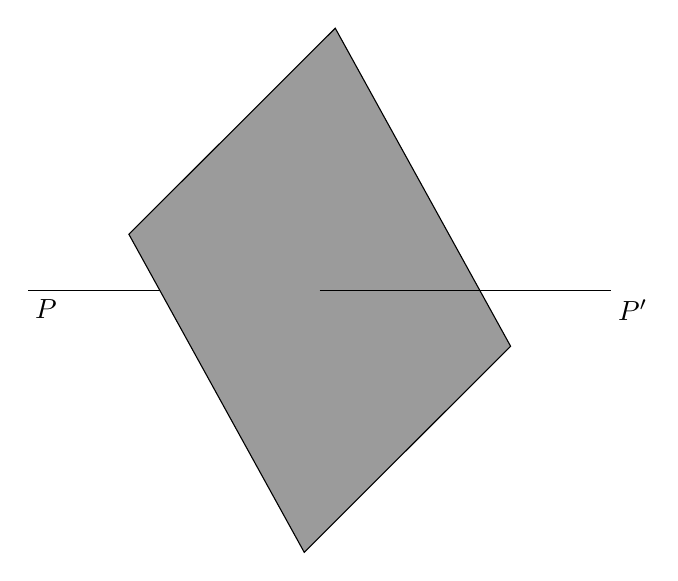
\begin{tikzpicture}[x=0.75pt,y=0.75pt,yscale=-1,xscale=1]
%uncomment if require: \path (0,300); %set diagram left start at 0, and has height of 300

%Straight Lines [id:da3197702069809195]
\draw    (155.65,146.42) -- (296.1,146.42) ;
%Shape: Rectangle [id:dp5114890032601768]
\draw  [fill={rgb, 255:red, 155; green, 155; blue, 155 }  ,fill opacity=1 ] (303.57,20.17) -- (388.06,173.4) -- (288.63,272.67) -- (204.14,119.43) -- cycle ;
%Straight Lines [id:da7013912332146902]
\draw    (296.1,146.42) -- (436.54,146.42) ;

% Text Node
\draw (157.65,149.82) node [anchor=north west][inner sep=0.75pt]    {$P$};
% Text Node
\draw (438.54,149.82) node [anchor=north west][inner sep=0.75pt]    {$P'$};


\end{tikzpicture}
\caption{Punto simétrico respecto a un plano}
\end{figure}
\begin{defin}
Sea $(A,V, \phi)$ un espacio afín sobre un cuerpo $\mathbb{K}$. Consideramos un subespacio afín $L$ de $A$ con dirección $W$ y un subespacio $U$ de $V$ complementario de $W$ $(U \bigoplus W = V)$. Llamamos simetría respecto de $L$ con dirección $U$ a la aplicación $\sigma$:
\begin{equation}
	\begin{split}
		\sigma: A &\to A\\
		P &\to P +2 \overline{P \delta(P)}
	\end{split}
\end{equation}
\end{defin}
Tipos de simetría:
\begin{itemize}
	\item Central: respecto a un punto.
	\item Axial: respecto a una recta.
	\item Especular: respecto a un plano.
\end{itemize}
\section{Giros y rotaciones}
\begin{defin}
Sea un EAE y sea un punto $O \in A$. Una rotación  es una aplicación $g$ de $E$ en $E$ que deja fijo $O$ $(g(O) = O)$, y que tiene por aplicación lineal asociada un giro de ángulo $\theta$:
\begin{equation}
	\begin{split}
		g: E &\to E\\
		P &\to g(P) = O +t(\vb{OP})
	\end{split}
\end{equation}
Donde $t(\vb{OP})$ es el vector después de rotarlo un ángulo $\theta$ respecto a $O$.  
\end{defin}
Propiedades:
\begin{itemize}
	\item Una rotación es biyectiva.
	\item La composición de rotaciones es una rotación.
	\item El único punto fijo de un giro es su centro.
	\item La rotación viene determinada por la imagen de dos puntos.
	\item Las rotaciones conservan distancias y ángulos, por lo que son isometrías.
\end{itemize}
\begin{defin}
Fijado un semieje $r$ y un ángulo $\alpha$, el giro se construye como
\[
	X' = P + t_{\alpha}(\vb{PX})
\]
Es decir, giramos el punto $X$, un ángulo $\alpha$ alrededor del eje $r$.   
\end{defin}
Propiedades:
\begin{itemize}
	\item Una rotación es biyectiva.
	\item La composición es una rotación.
	\item Los puntos fijos son todos aquellos que pertenecen al eje.
	\item La orientación del giro viene determinada por el sentido del vector director de la recta.
\end{itemize}
\section{Puntos fijos}
\begin{defin}
Dado un EA, y $f$ una transformación afín de $A$, y $R=\{ O, \mathcal{B} \}$ un sistema de referencia de $A$. Sea la matriz asociada de $f$:
\[
	M_{R}(f) = \mqty(1 & 0 \\ a & \mathcal{M})
\]
donde $\mathcal{M}$ es la matriz asociada a la aplicación lineal $\bar{f}$ en la base $\mathcal{B}$. Todos los puntos fijos de $f$ satisfacen la ecuación:
\[
	O = (\mathcal{M} - I) \vb{OP}+a
\]
\end{defin}
\subsection{Clasificación}
La ecuación del subespacio de puntos fijos de $f$ es
\[
	(\mathcal{M}-I)X +a = O
\]
Definamos $M= (\mathcal{M}-I)$ y $M'=(\mathcal{M}-I)|a$.
\begin{itemize}
	\item Si $rg(M) =rg(M') = 2$, entonces $f$ tiene un único punto fijo.
	\item Si $rg(M) = rg(M') = 1$, entonces $f$ tiene una recta de puntos fijos.
	\item Si $rg(M) = rg(M') = 0$, entonces $f$ es la aplicación identidad.  
\end{itemize}
\begin{defin}
Una simetría deslizante es aquella que consiste en una traslación y una simetría axial paralela al eje de traslación.
\end{defin}
\end{document}
